\chapter{LITERATURE REVIEW}
\label{chap:2}

\section{Myocardial Infarction}
\label{sec:mi}

Myocardial infarction (MI), commonly known as a heart attack, is one of the leading causes of morbidity and mortality worldwide. It occurs when blood flow through a coronary artery is partially or completely blocked, resulting in prolonged oxygen deprivation of the heart muscle. If blood supply is not restored promptly, irreversible damage to the myocardium occurs, leading to the formation of non-contractile scar tissue and permanent impairment of cardiac function \citep{Thygesen2019}.

Following myocardial infarction, the damaged myocardium undergoes a healing process in which necrotic tissue is gradually replaced by fibrotic scar tissue. Unlike healthy myocardium, scar tissue has little or no contractile capability, reducing the pumping efficiency of the left ventricle. Extensive myocardial scarring has been associated with ventricular remodeling, heart failure, life-threatening arrhythmias, and an increased risk of sudden cardiac death \citep{Thygesen2019,Ibanez2018}.

\begin{figure}[htbp]
	\centering
	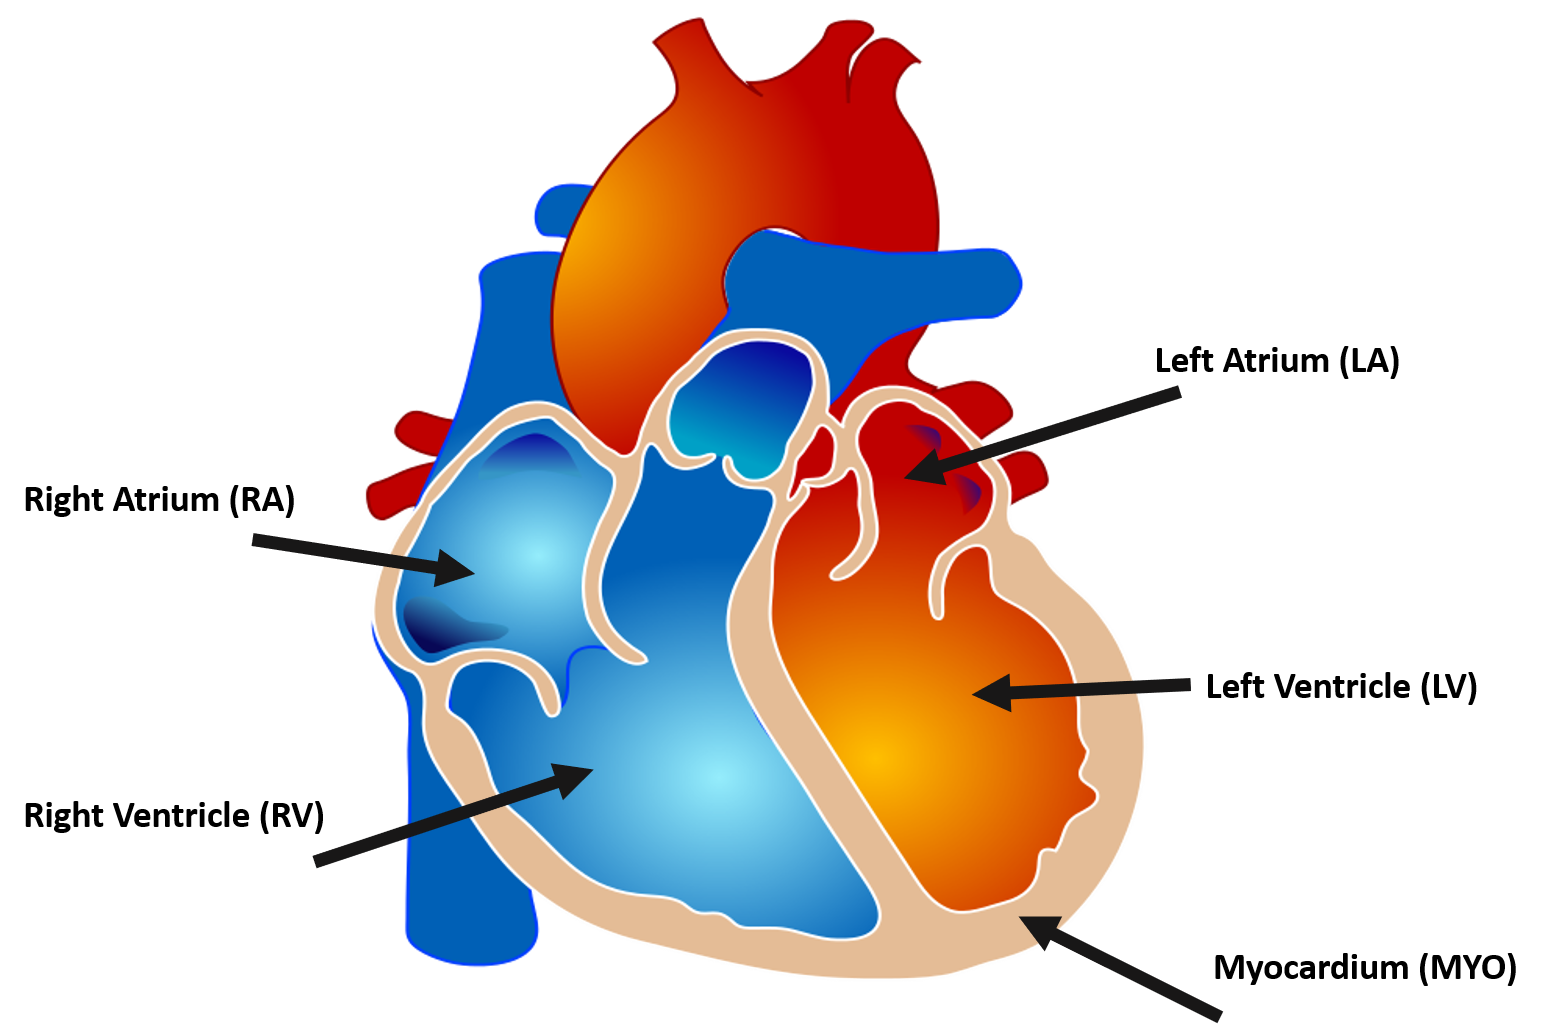
\includegraphics[width=0.86\textwidth]{bab2/ch2-heart-anatomy.png}
	\caption{Anatomy of the human heart \citep{Shade2013}}
	\label{fig:ch2-heart-anatomy}
\end{figure}

Figure~\ref{fig:ch2-heart-anatomy} illustrates the basic anatomy of the heart, including the left ventricle, right ventricle, atria, and myocardium. Among these structures, the myocardium is the primary region affected by myocardial infarction and therefore becomes the main focus of this dissertation.

\begin{figure}[htbp]
	\centering
	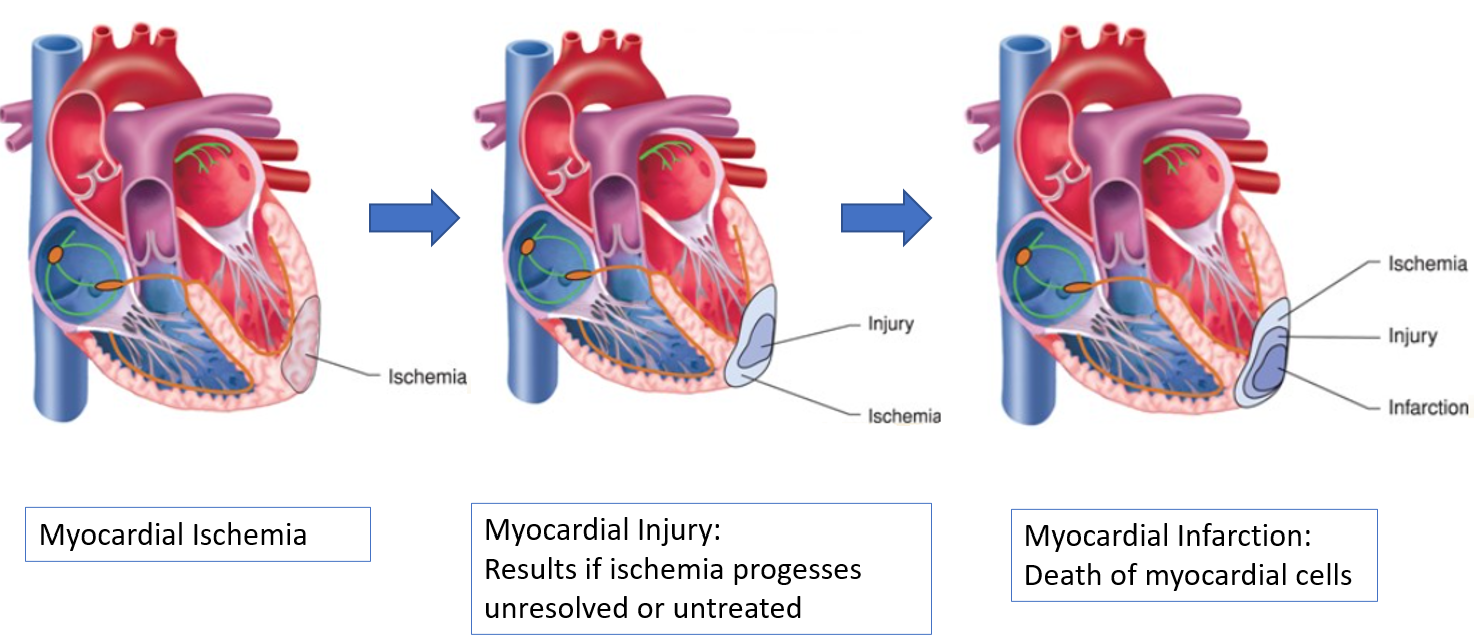
\includegraphics[width=0.86\textwidth]{bab2/ch2-mi-development.png}
	\caption{Development of myocardial infarction following prolonged coronary artery obstruction \citep{Shade2013}}
	\label{fig:ch2-mi-development}
\end{figure}

As illustrated in Figure~\ref{fig:ch2-mi-development}, prolonged interruption of blood supply causes myocardial cells to lose oxygen and nutrients, eventually resulting in irreversible tissue injury. During the healing process, the damaged myocardium is replaced by fibrotic scar tissue, which permanently alters the mechanical function of the heart.

\begin{figure}[htbp]
	\centering
	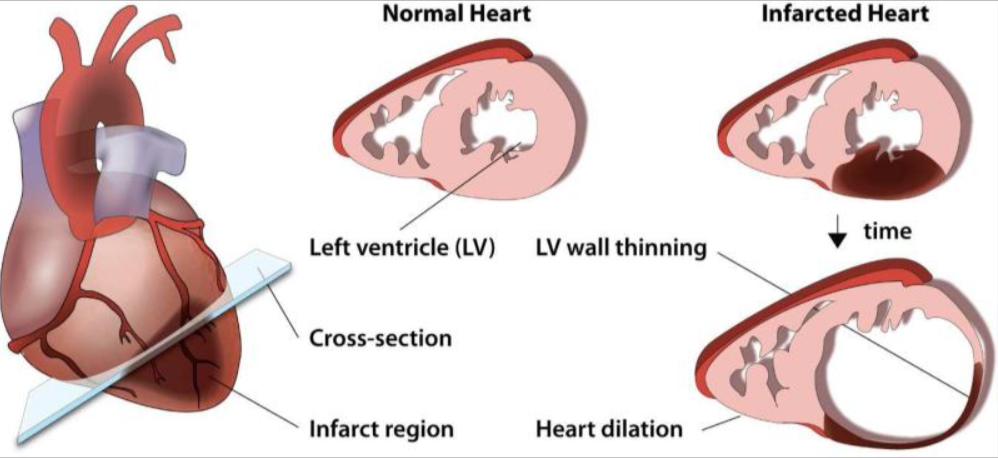
\includegraphics[width=0.86\textwidth]{bab2/ch2-healthy-infarcted.png}
	\caption{Comparison of healthy and infarcted myocardium \citep{Awada2016}}
	\label{fig:ch2-healthy-infarcted}
\end{figure}

The extent and location of myocardial scar are closely related to cardiac function and clinical outcome. Consequently, accurate assessment of myocardial scar has become an essential component in the diagnosis, treatment planning, and follow-up of patients with myocardial infarction. Reliable scar quantification provides valuable information for evaluating infarct severity, predicting functional recovery, and supporting therapeutic decision-making \citep{Kim2000,Ibanez2018}.

Although several imaging modalities are available for cardiac assessment, each has different strengths and limitations in visualizing myocardial tissue. Among these modalities, CMR has emerged as the reference standard because it enables comprehensive evaluation of cardiac anatomy, ventricular function, and myocardial tissue characteristics within a single examination. Therefore, the following section reviews the principles and clinical advantages of CMR for myocardial infarction assessment.

\section{Cardiac Magnetic Resonance Imaging}
\label{sec:cmr}

Cardiac Magnetic Resonance (CMR) has become one of the most important imaging modalities for the evaluation of cardiovascular diseases because it provides comprehensive information on cardiac anatomy, ventricular function, tissue characterization, and myocardial viability without exposing patients to ionizing radiation. Compared with echocardiography, computed tomography (CT), and nuclear imaging, CMR offers superior soft tissue contrast and high spatial resolution, making it particularly suitable for myocardial infarction assessment \citep{Kramer2020,Pennell2010}.

CMR examinations can be performed using different imaging sequences, each providing complementary clinical information. Among these, cine CMR is widely used to evaluate cardiac morphology and ventricular function, whereas Late Gadolinium Enhancement (LGE) imaging is considered the clinical reference for detecting myocardial scar. The combination of these imaging sequences enables both functional and structural assessment of the myocardium within a single examination \citep{Kramer2020}.

\begin{figure}[htbp]
	\centering
	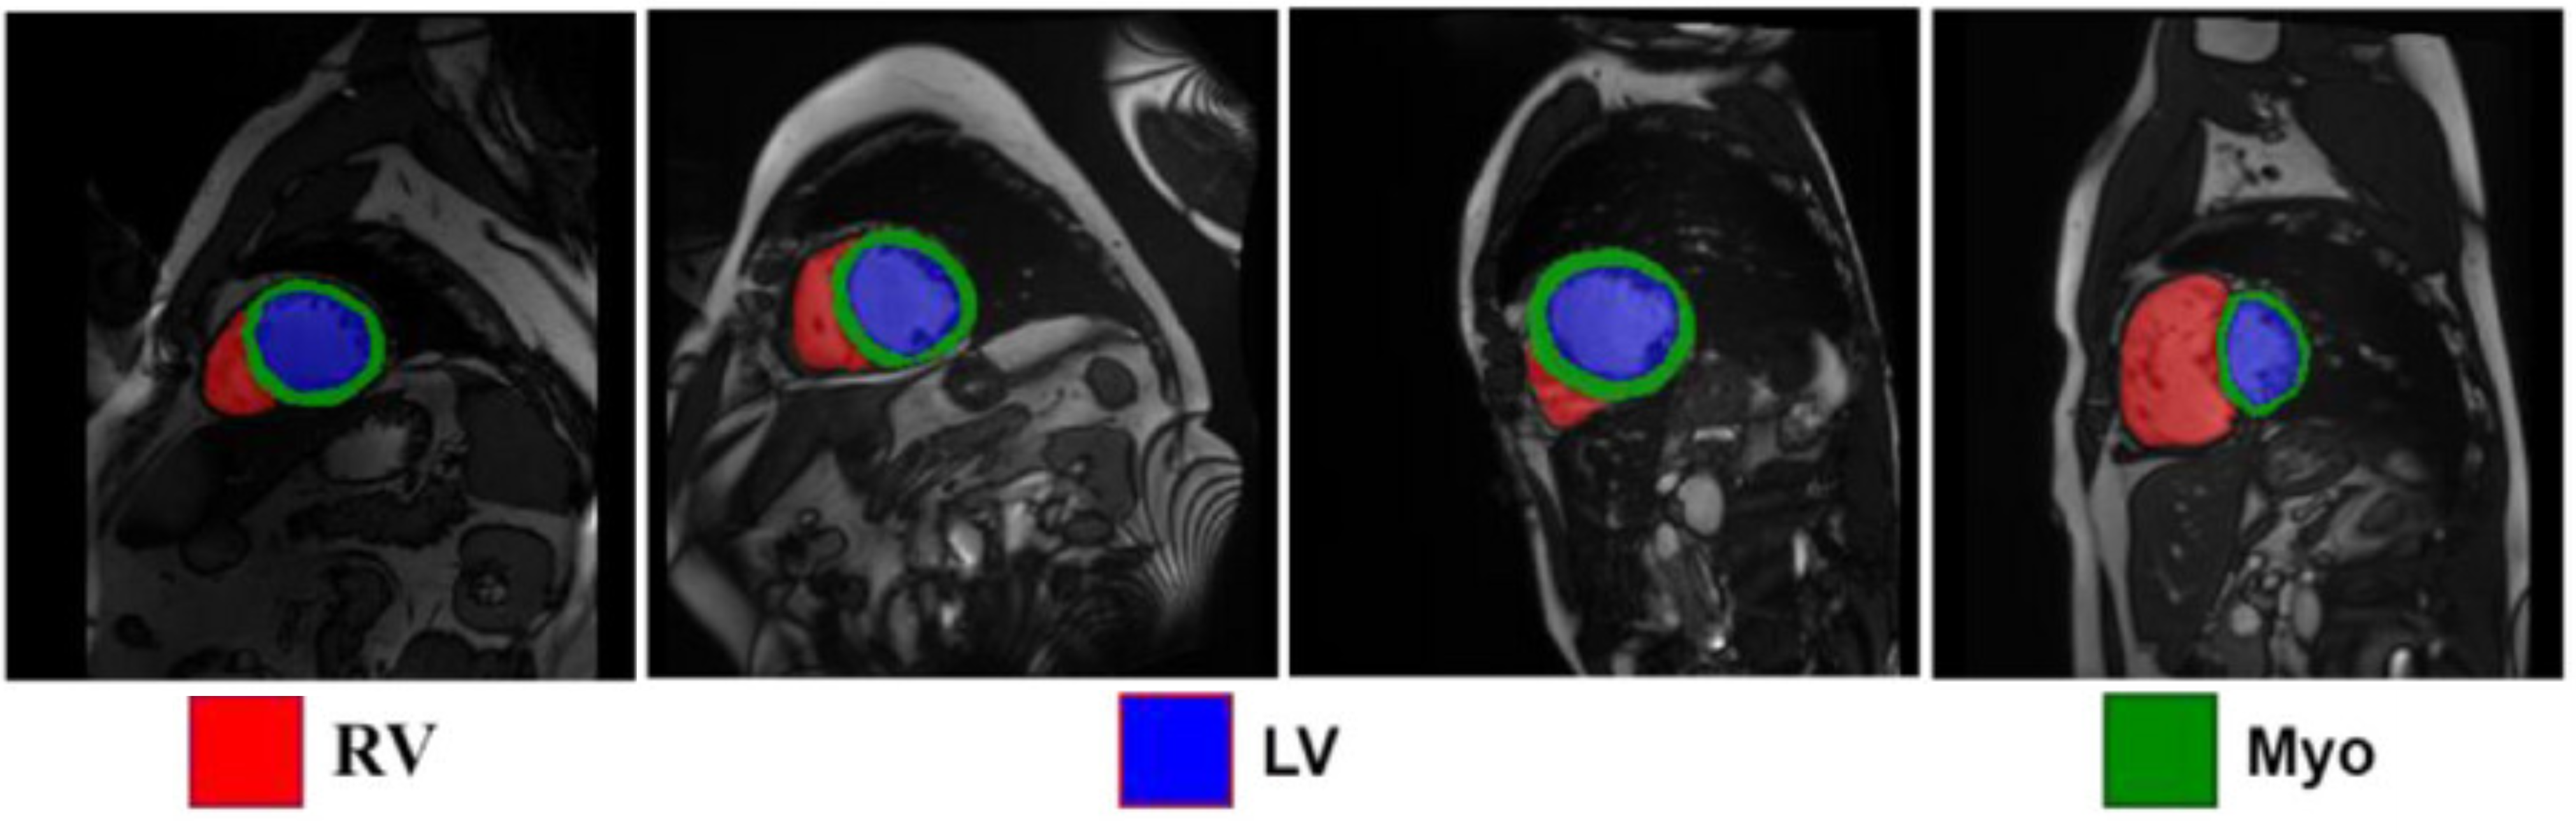
\includegraphics[width=0.86\textwidth]{bab2/ch2-cmr-sequences.png}
	\caption{Representative CMR imaging sequences used for myocardial infarction assessment \citep{Xie2024}}
	\label{fig:ch2-cmr-sequences}
\end{figure}

Figure~\ref{fig:ch2-cmr-sequences} illustrates the complementary information provided by different CMR sequences. Cine CMR clearly visualizes cardiac chambers and myocardial motion throughout the cardiac cycle, whereas LGE highlights infarcted myocardium by exploiting differences in gadolinium contrast uptake between healthy and damaged tissues. Consequently, both sequences provide essential information for comprehensive myocardial infarction assessment.

\subsection{Cine Cardiac Magnetic Resonance Imaging}
\label{subsec:cine-cmr}

Cine CMR produces a series of images acquired throughout the cardiac cycle, allowing dynamic visualization of cardiac motion. It is widely used to evaluate ventricular size, myocardial thickness, wall motion, and global cardiac function. Because of its excellent contrast between the blood pool and myocardium, cine CMR has become the standard imaging modality for automatic segmentation of the left ventricle, right ventricle, and myocardium \citep{Petitjean2011,Bernard2018}.

The availability of publicly accessible datasets has further accelerated the development of automated cardiac structure segmentation. One of the most widely used benchmark datasets is the Automated Cardiac Diagnosis Challenge (ACDC) dataset, which provides cine CMR images together with expert annotations of the left ventricle, right ventricle, and myocardium at end-diastole and end-systole. This dataset has become a standard benchmark for evaluating deep learning algorithms in cardiac image segmentation \citep{Bernard2018}.

\subsection{Multi-Sequence Cardiac Magnetic Resonance Imaging}
\label{subsec:multi-sequence}

While cine CMR primarily provides anatomical and functional information, myocardial infarction assessment also requires characterization of pathological changes within the myocardial tissue. Late Gadolinium Enhancement (LGE) imaging is particularly important for this purpose. Following intravenous administration of a gadolinium-based contrast agent, normal myocardium rapidly washes out the contrast material, whereas infarcted or fibrotic tissue retains gadolinium for a longer period. Consequently, damaged myocardial tissue appears hyperintense relative to healthy myocardium, making LGE an established imaging technique for myocardial scar visualization (Kim et al., 1999; Kramer et al., 2020).

For more comprehensive myocardial tissue characterization, multiple CMR sequences can be combined to provide complementary information. Multi-sequence CMR commonly integrates balanced steady-state free precession (bSSFP), T2-weighted imaging (T2WI), and LGE. The bSSFP sequence provides anatomical and functional information, T2WI is sensitive to myocardial edema, whereas LGE highlights irreversible myocardial injury and fibrotic scar tissue. Combining these sequences therefore provides richer information for myocardial pathology assessment than relying on a single sequence alone (Zhuang, 2019).

The Myocardial Pathology Segmentation (MyoPS) dataset provides an important benchmark for this type of analysis. It contains co-registered bSSFP, T2-weighted, and LGE images together with expert annotations of myocardial structures and pathological regions, including myocardial scar. 
This multi-sequence representation enables automated methods to exploit complementary anatomical and tissue-characterization information for myocardial pathology segmentation (Zhuang, 2019).

Overall, cine and multi-sequence CMR serve complementary roles in the analysis performed in this dissertation. Cine CMR provides the anatomical information required for cardiac structure segmentation, whereas multi-sequence CMR, particularly LGE, provides the tissue information 
required for myocardial scar assessment. The characteristics and clinical significance of myocardial scar are discussed in the following section.

\section{Myocardial Scar Assessment}
\label{sec:scar-assessment}

Myocardial scar assessment plays an important role in the clinical management of myocardial infarction because the extent and distribution of scar tissue are closely associated with cardiac function and patient prognosis. Following myocardial infarction, damaged myocardial cells are gradually replaced by fibrotic tissue that permanently alters the mechanical and electrical properties of the heart. Consequently, accurate identification and quantification of myocardial scar provide valuable information for evaluating infarct severity, predicting ventricular remodeling, and supporting therapeutic decision-making \citep{Kim1999,Kramer2020}.

\subsection{Myocardial Scar}
\label{subsec:myocardial-scar}

Myocardial scar is formed as part of the natural healing process after irreversible injury to the heart muscle. Unlike healthy myocardium, scar tissue has little or no contractile capability because it consists primarily of fibrotic tissue rather than functional cardiac muscle cells. The presence of myocardial scar reduces ventricular contractility and may contribute to impaired cardiac performance, heart failure, and ventricular arrhythmias \citep{Ibanez2018}.

The appearance of myocardial scar on CMR depends on the imaging sequence used. In Late Gadolinium Enhancement (LGE) images, example from MyoPS dataset, scar tissue appears brighter than healthy myocardium because fibrotic tissue retains gadolinium contrast agents for a longer period. This difference in signal intensity enables myocardial scar to be identified with high sensitivity and has established LGE as the clinical reference standard for infarct visualization \citep{Kim1999}.

\begin{figure}[htbp]
	\centering
	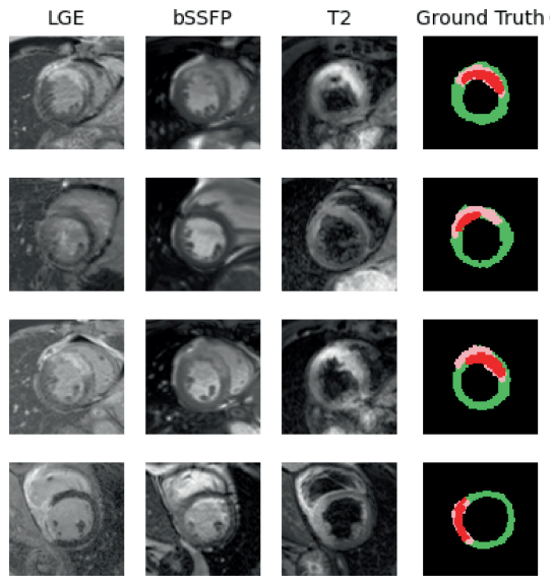
\includegraphics[width=0.86\textwidth]{bab2/ch2-lge-scar.png}
	\caption{Representative LGE-CMR image showing myocardial scar \citep{Margolis2025}}
	\label{fig:ch2-lge-scar}
\end{figure}

Figure~\ref{fig:ch2-lge-scar} illustrates the appearance of myocardial scar in an LGE-CMR image. The hyperenhanced region corresponds to infarcted myocardium, whereas the surrounding darker region represents healthy myocardial tissue. Accurate identification of these regions is essential for reliable myocardial infarction assessment.

\subsection{Clinical Significance of Myocardial Scar Assessment}
\label{subsec:clinical-scar}

Beyond identifying the presence of infarction, myocardial scar assessment provides clinically important information regarding the severity of myocardial damage. Previous studies have demonstrated that larger scar burden is associated with poorer ventricular function, lower recovery potential after revascularization, and an increased risk of adverse cardiac events \citep{Kim2000,Ibanez2018}.

In clinical practice, scar assessment is generally performed by manually outlining infarcted regions on LGE images. Although manual analysis is widely accepted, it is labor-intensive, requires experienced clinicians, and is subject to inter- and intra-observer variability. These limitations become more pronounced when scar boundaries are indistinct or when infarct morphology varies considerably among patients.

\subsection{Automated Myocardial Scar Segmentation}
\label{subsec:auto-scar}

To overcome the limitations of manual analysis, numerous automated and deep learning-based segmentation methods have been proposed. Recent studies have shown that convolutional neural networks, particularly U-Net-based architectures, can accurately identify myocardial scar while substantially reducing analysis time \citep{Oktay2018,Isensee2018}.

The availability of public benchmark datasets has further accelerated research in this area. In particular, the Myocardial Pathology Segmentation (MyoPS) dataset provides standardized multi-sequence CMR images with expert annotations, enabling objective comparison of automated segmentation algorithms under consistent evaluation protocols \citep{Zhuang2019}.

Although considerable progress has been achieved, automated myocardial scar segmentation remains a challenging task. Scar regions often exhibit large variations in size, shape, and image intensity, while the contrast between scar tissue and surrounding myocardium may be weak in some patients. These challenges continue to motivate the development of more reliable deep learning approaches for CMR image analysis.

Besides accurate scar segmentation, effective myocardial infarction assessment also depends on the ability of deep learning models to learn robust image representations. Therefore, the following section reviews the development of artificial intelligence and deep learning techniques for medical image analysis before discussing the segmentation architectures adopted in this dissertation.

\section{Deep Learning in Cardiac Magnetic Resonance Imaging}
\label{sec:dl-cmr}

The growing use of CMR imaging has generated a large amount of imaging data that requires accurate and efficient analysis. Traditionally, cardiac structures and myocardial abnormalities were identified manually by experienced clinicians. Although manual interpretation remains the clinical reference, it is time-consuming, requires substantial expertise, and may produce variations between observers, particularly when image quality is poor or tissue boundaries are difficult to identify \citep{Petitjean2011,Kramer2020}.

To improve efficiency and consistency, researchers initially developed computer-assisted image analysis based on conventional image processing and machine learning techniques. These approaches relied on manually designed features such as image intensity, texture, shape, and edge information before classification or segmentation could be performed. While these methods showed promising results, their performance depended heavily on feature selection and often struggled to handle the large variability found in cardiac MR images \citep{Litjens2017}.

The rapid development of deep learning has significantly changed the way medical images are analyzed. Unlike conventional machine learning, deep learning automatically learns relevant image features directly from training data without requiring manual feature engineering. This capability enables the model to recognize complex anatomical structures and tissue characteristics more effectively, leading to substantial improvements in medical image segmentation performance \citep{LeCun2015,Litjens2017}.

Among various deep learning approaches, Convolutional Neural Networks (CNNs) have become the foundation of most medical image analysis systems. CNNs learn hierarchical image features through convolutional operations, allowing both low-level image patterns and high-level anatomical structures to be represented automatically. As a result, CNN-based methods have demonstrated superior performance in many medical imaging applications, including organ segmentation, lesion detection, disease classification, and image reconstruction \citep{LeCun2015,Shen2017}.

The success of CNNs also accelerated the development of semantic segmentation networks specifically designed for pixel-level image analysis. One important milestone was the introduction of Fully Convolutional Networks (FCNs), which replaced fully connected layers with convolutional layers to generate dense segmentation maps directly from input images. FCNs demonstrated that deep learning could perform end-to-end image segmentation without requiring handcrafted post-processing, opening new opportunities for automated medical image analysis \citep{Long2015}.

Building upon the FCN concept, U-Net was specifically designed for biomedical image segmentation by integrating an encoder--decoder structure with skip connections to preserve fine spatial and anatomical details during feature reconstruction. Owing to its high segmentation accuracy and relatively simple architecture, U-Net has become the most widely adopted backbone for cardiac MR image segmentation and has inspired numerous architectural improvements for different clinical applications \citep{Ronneberger2015,Siddique2021}.

Given its extensive use in cardiac image analysis, understanding the architecture and characteristics of U-Net is essential before discussing more specific components, such as activation functions, pooling strategies, loss functions, residual learning, and attention mechanisms. Therefore, the following section reviews the U-Net architecture as the foundation of many deep learning-based cardiac image segmentation methods.

\section{U-Net Architecture}
\label{sec:unet}

Among various deep learning architectures developed for image segmentation, U-Net has become one of the most widely adopted models in biomedical image analysis. Proposed by \citep{Ronneberger2015}, U-Net was specifically designed to perform accurate pixel-level segmentation using relatively limited training data. Owing to its simple architecture and robust performance, U-Net has been successfully applied to numerous medical imaging applications, including organ segmentation, tumor detection, retinal vessel extraction, brain lesion analysis, and CMR image segmentation \citep{Ronneberger2015,Siddique2021}.

The U-Net architecture consists of two main components, namely an encoder and a decoder, which are connected through skip connections. The encoder progressively extracts increasingly abstract image features while reducing the spatial resolution through convolution and pooling operations. In contrast, the decoder gradually restores the spatial resolution using upsampling operations to generate a pixel-wise segmentation map. Skip connections directly transfer feature information from the encoder to the corresponding decoder layers, allowing fine anatomical details to be preserved during image reconstruction \citep{Ronneberger2015}.

\begin{comment}
Figure~\ref{fig:ch2-unet-architecture} illustrates the overall architecture of U-Net. The encoder learns hierarchical image features from low-level visual patterns to high-level semantic representations, whereas the decoder reconstructs these features into a segmentation map with the same spatial resolution as the input image. The skip connections play an important role in preserving spatial information by combining low-level and high-level features, enabling accurate localization of anatomical structures.

\begin{figure}[htbp]
	\centering
	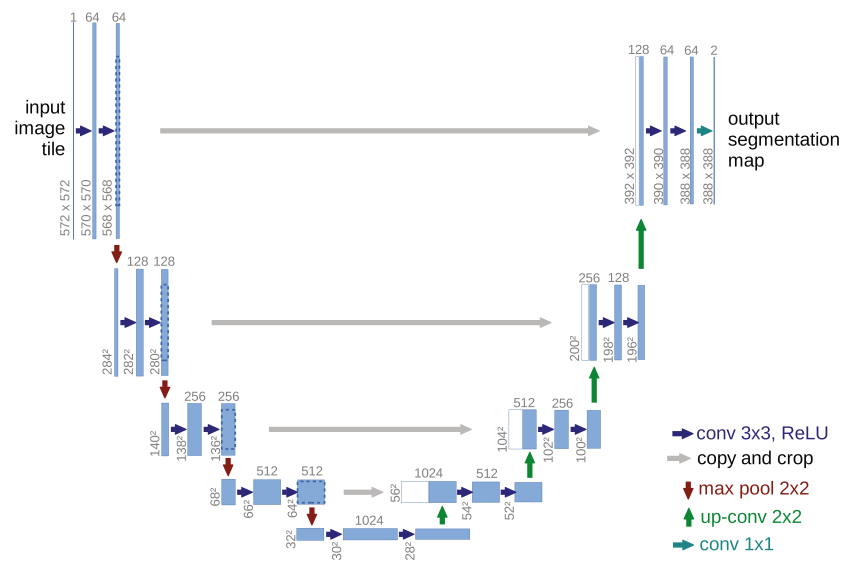
\includegraphics[width=0.75\textwidth]{bab2/ch2-unet-architecture.png}
	\caption{General architecture of U-Net for biomedical image segmentation \citep{Ronneberger2015}}
	\label{fig:ch2-unet-architecture}
\end{figure}
\end{comment}

Because of these advantages, U-Net has become the baseline architecture for many CMR image segmentation studies. It has demonstrated excellent performance in segmenting the left ventricle, right ventricle, and myocardium from cine CMR images, making it one of the most widely adopted architectures in cardiovascular image analysis \citep{Petitjean2011,Bernard2018}.

Despite its success, the segmentation performance of U-Net is still influenced by several components within the network architecture. Previous studies have shown that activation functions affect nonlinear feature learning, pooling mechanisms influence spatial information preservation, and loss functions determine how the network learns from prediction errors during training. In addition, more advanced feature learning strategies have been introduced to further improve segmentation accuracy in challenging medical images. Therefore, these architectural components are reviewed in the following sections as the theoretical foundation for the methods developed in this dissertation.

\section{Activation Functions for Medical Image Segmentation}
\label{sec:activation-functions}

Activation functions are fundamental components of deep neural networks because they introduce nonlinear transformations that enable the network to learn complex feature representations from image data. Without nonlinear activation functions, multiple convolutional layers would behave as a linear transformation, substantially limiting the representational capability of deep neural networks. Consequently, activation functions play an important role in feature extraction, training stability, gradient propagation, and convergence behaviour during network training \citep{Nair2010,Nwankpa2018}.

In medical image segmentation, the influence of activation functions becomes increasingly important because anatomical structures often exhibit low contrast, indistinct boundaries, and considerable morphological variability. These characteristics are particularly evident in CMR images, where accurate segmentation of the left ventricle, right ventricle, and myocardium depends on the network's ability to learn discriminative image features while maintaining stable learning throughout training \citep{Chen2020Review,Hesamian2019}.

Among the numerous activation functions proposed for deep learning, the Rectified Linear Unit (ReLU) has become the most widely adopted because of its computational simplicity and effective mitigation of the vanishing-gradient problem. ReLU preserves positive activation values while suppressing negative responses, thereby facilitating efficient gradient propagation and accelerating network convergence \citep{Nair2010}. The ReLU activation function is defined as

\begin{equation}
	f(x)=\max(0,x)
	\label{eq:relu}
\end{equation}

where $x$ denotes the input activation.

Despite its widespread adoption, ReLU is not without limitations. Since all negative input values are mapped to zero, neurons receiving predominantly negative activations may become permanently inactive during training, a phenomenon commonly referred to as the dying ReLU problem. This limitation may reduce feature diversity and affect segmentation performance, particularly when anatomical boundaries are weak or tissue contrast is limited.

To overcome these limitations, several alternative activation functions have been proposed. One of the most promising is Mish, a smooth self-regularized non-monotonic activation function that preserves a portion of negative activation values while maintaining continuous gradient propagation \citep{Misra2020}. Compared with ReLU, Mish is expected to provide richer feature representation and smoother training behaviour in deep neural networks.

The Mish activation function is expressed as
\begin{equation}
	f(x) = x \tanh\left(\operatorname{softplus}(x)\right),
	\label{eq:mish}
\end{equation}%
where
\begin{equation}
	\operatorname{softplus}(x) = \ln(1+e^x).
	\label{eq:softplus}
\end{equation}

Figure~\ref{fig:ch2-activation-comparison} illustrates the characteristics of the ReLU and Mish activation functions. ReLU generates zero output for all negative inputs while maintaining a linear response for positive values. In contrast, Mish produces a smooth nonlinear response that preserves a portion of negative activations, allowing richer information flow during feature learning. These different characteristics may influence feature representation capability and segmentation performance in deep neural networks.

\begin{figure}[htbp]
	\centering
	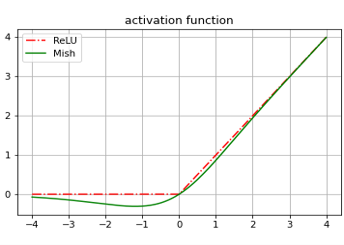
\includegraphics[width=0.62\textwidth]{bab2/ch2-activation-comparison.png}
	\caption{Comparison of the ReLU and Mish activation functions \citep{Riandini2022IST}}
	\label{fig:ch2-activation-comparison}
\end{figure}

Overall, activation functions directly influence how discriminative image features are learned throughout the training process. Since CMR segmentation requires accurate delineation of complex cardiac structures with subtle anatomical boundaries, selecting an appropriate activation function represents an important consideration in improving segmentation performance. Besides activation functions, another fundamental component that strongly influences feature representation is the pooling mechanism used during feature downsampling. Therefore, the following section reviews pooling mechanisms commonly employed in deep learning-based medical image segmentation.

\section{Pooling Mechanisms for Medical Image Segmentation}
\label{sec:pooling}

Pooling is an essential operation in convolutional neural networks because it reduces the spatial dimensions of feature maps while preserving representative image information. By progressively reducing the feature map size, pooling decreases computational complexity, enlarges the receptive field, and improves computational efficiency. Consequently, pooling has become a fundamental component of deep learning models for medical image segmentation \citep{Goodfellow2016,Chen2020Review}.

Among the available pooling strategies, Max Pooling is the most widely adopted because of its simple implementation and computational efficiency. During the pooling process, only the largest activation value within a local neighborhood is retained, while the remaining activation values are discarded. This operation effectively preserves the most dominant feature response and is mathematically defined as

\begin{equation}
	P_{\max}=\max(x_1,x_2,\ldots,x_n)
	\label{eq:max-pooling}
\end{equation}

where $x_i$ represents the activation values within a pooling window.

Although Max Pooling has demonstrated satisfactory performance in many segmentation tasks, retaining only the maximum activation may discard useful local information. This limitation becomes particularly important in CMR image segmentation because the myocardium appears as a relatively thin structure with subtle anatomical boundaries. As a result, repeated downsampling may gradually reduce boundary information and affect segmentation accuracy.

To overcome this limitation, several alternative pooling strategies have been proposed. One of these is Fuzzy Logic-Based Pooling, which incorporates fuzzy set theory into the pooling process by assigning a membership value to each activation before computing the pooled feature. Instead of selecting only the strongest activation, fuzzy pooling allows information from all activation values to contribute to the pooled representation according to their corresponding membership coefficients. This strategy preserves richer local contextual information while reducing information loss during feature downsampling \citep{Zadeh1965,Diamantis2020}.

The generalized fuzzy pooling operation is expressed as

\begin{equation}
	P_{\mathrm{fuzzy}}=\frac{\sum_{i=1}^{n}\mu_i x_i}{\sum_{i=1}^{n}\mu_i}
	\label{eq:fuzzy-pooling}
\end{equation}

where $x_i$ denotes the activation value, $\mu_i$ represents the corresponding fuzzy membership coefficient, and $n$ denotes the number of activation values within the pooling window.

\begin{comment}
\begin{figure}[htbp]
	\centering
	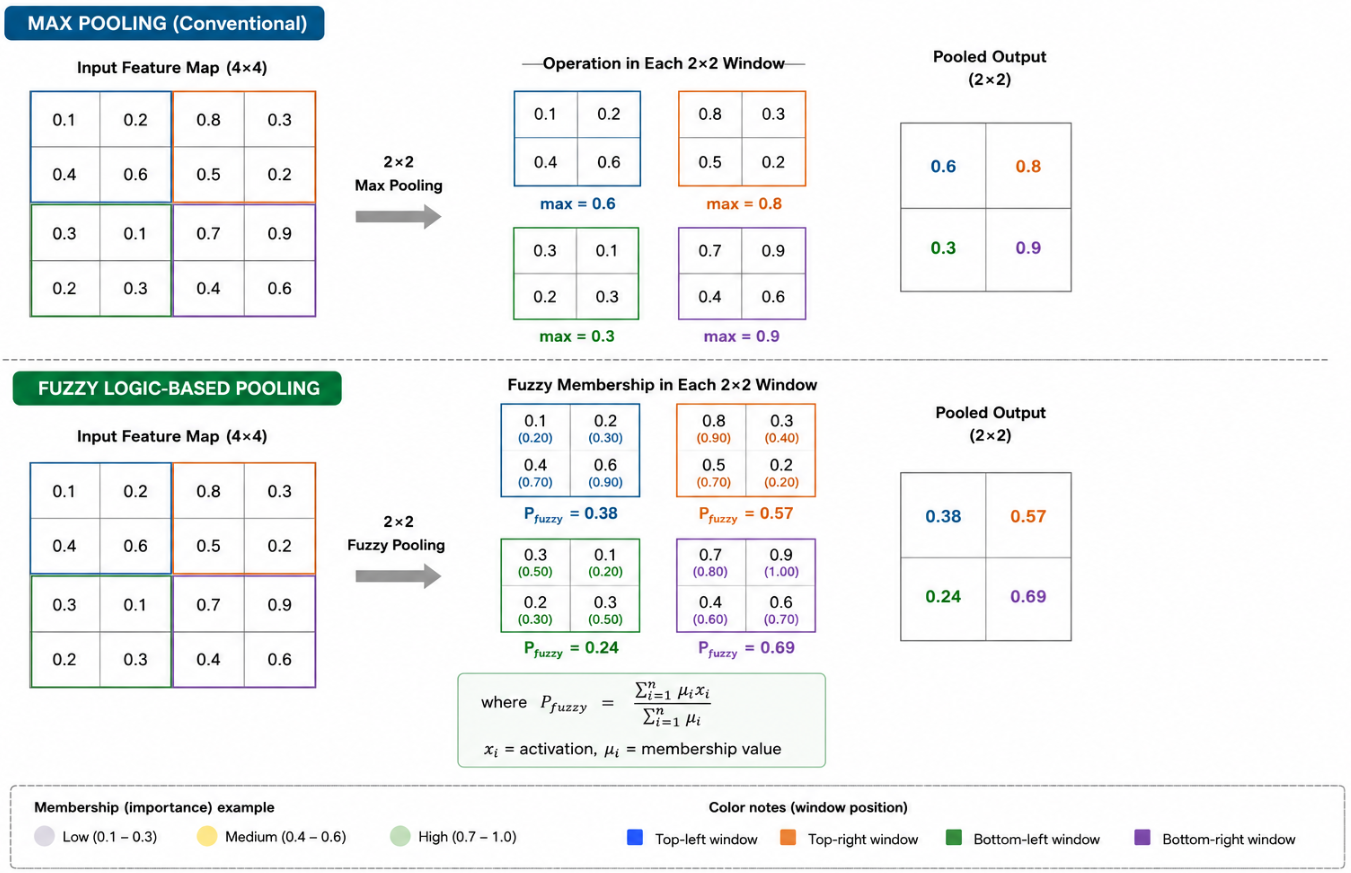
\includegraphics[width=0.86\textwidth]{bab2/ch2-pooling-comparison.png}
	\caption{Example of comparison between conventional max pooling and fuzzy logic-based pooling}
	\label{fig:ch2-pooling-comparison}
\end{figure}

Figure~\ref{fig:ch2-pooling-comparison} illustrates the conceptual difference between the two pooling strategies. Max Pooling preserves only the strongest activation within each pooling window, whereas Fuzzy Logic-Based Pooling aggregates information from all activation values according to their membership coefficients. Consequently, fuzzy pooling is able to preserve richer spatial information and better maintain anatomical continuity during feature extraction.
\end{comment}

Overall, the pooling mechanism has a direct influence on feature representation learned by deep neural networks. Since accurate CMR segmentation depends on preserving thin myocardial boundaries and subtle anatomical structures, selecting an appropriate pooling strategy remains an important consideration for improving segmentation performance. Besides feature extraction, segmentation performance is also influenced by the learning objective used during network training. Therefore, the following section reviews the loss functions commonly employed in deep learning-based medical image segmentation.

\section{Loss Functions for Medical Image Segmentation}
\label{sec:loss-functions}

Loss functions play a fundamental role in deep learning because they measure the discrepancy between the predicted output and the corresponding ground-truth annotation during network training. The computed loss is subsequently minimized through backpropagation, enabling the network to progressively improve its segmentation performance. Consequently, the choice of an appropriate loss function directly influences learning behaviour, convergence stability, and the final segmentation accuracy \citep{Jadon2020,Ma2021}.

In medical image segmentation, selecting an appropriate loss function is particularly important because the target anatomy often occupies only a small portion of the image. Under such conditions, conventional loss functions may become dominated by background pixels, making it difficult for the network to accurately learn small anatomical structures and object boundaries. To address this challenge, various loss functions have been developed, each emphasizing different learning objectives.

One of the most widely used objective functions is Cross-Entropy Loss, which evaluates the difference between the predicted class probabilities and the corresponding ground-truth labels. Because of its simple formulation and stable training behaviour, Cross-Entropy Loss has become the standard objective function for many image classification and segmentation tasks.

The Cross-Entropy Loss is defined as

\begin{equation}
	\mathcal{L}_{\mathrm{CE}}=-\sum_{i=1}^{C} y_i\log(\hat{y}_i)
	\label{eq:cross-entropy}
\end{equation}

where $y_i$ denotes the ground-truth label, $\hat{y}_i$ represents the predicted probability, and $C$ is the total number of classes.

Although Cross-Entropy Loss performs well for balanced datasets, its effectiveness may decrease when the target object occupies only a limited image area. Consequently, several overlap-based loss functions have been introduced for medical image segmentation.

Among these, Dice Loss has become one of the most commonly adopted because it directly maximizes the overlap between the predicted segmentation and the reference annotation. Since Dice Loss focuses on region similarity rather than individual pixel classification, it is generally more robust to class imbalance than Cross-Entropy Loss \citep{Milletari2016}.

Another widely adopted objective function is Focal Loss, which extends Cross-Entropy Loss by assigning greater weight to difficult training samples while reducing the contribution of easily classified pixels. This enables the network to focus more effectively on small or challenging regions that are frequently misclassified \citep{Lin2017}.

To further improve segmentation overlap, Lov\'asz-Softmax Loss was proposed as a differentiable surrogate for the Intersection over Union (IoU) metric. Unlike conventional pixel-wise loss functions, Lov\'asz-Softmax directly improves segmentation overlap, making it particularly suitable for semantic segmentation tasks in which IoU is used as the primary evaluation metric \citep{Berman2018}.

\begin{table}[htbp]
	\centering
	\caption{Comparison of representative loss functions for medical image segmentation} %\cite{Berman2018,Jadon2020,Lin2017,Milletari2016}}
	\label{tab:loss-functions}
	
	\small
	\renewcommand{\arraystretch}{1.2}
	\begin{tabular}{
			>{\raggedright\arraybackslash}p{0.18\textwidth}
			>{\raggedright\arraybackslash}p{0.27\textwidth}
			>{\raggedright\arraybackslash}p{0.27\textwidth}
			>{\raggedright\arraybackslash}p{0.20\textwidth}
		}
		\toprule
		\textbf{Loss Function} & \textbf{Main Characteristic} & \textbf{Strength} & \textbf{Limitation} \\ \midrule
		Cross-Entropy & Pixel-wise classification & Stable training and simple implementation & Sensitive to class imbalance \\
		Dice Loss & Region overlap & Effective for imbalanced segmentation tasks & May be less stable during early training \\
		Focal Loss & Weighted learning of difficult samples & Improves learning of small target regions & Requires additional parameter tuning \\
		Lov\'asz-Softmax & Direct optimization of IoU & Improves region overlap & Higher computational complexity \\ \bottomrule
	\end{tabular}
	
	\vspace{4pt}
	{\raggedright \footnotesize \textit{Source:} Adapted from \cite{Milletari2016}, \cite{Lin2017}, \cite{Berman2018}, and \cite{Jadon2020}.\par}
\end{table}

Table~\ref{tab:loss-functions} summarizes the characteristics of the most widely used loss functions for medical image segmentation. Each loss function emphasizes a different learning objective and therefore exhibits different training behaviour. Consequently, selecting an appropriate loss function should consider the characteristics of the segmentation task, including class imbalance, object size, boundary complexity, and the evaluation metric used.

Overall, previous studies demonstrate that no single loss function consistently achieves the best performance across all segmentation tasks. Instead, the effectiveness of a loss function depends on the characteristics of the image data and the anatomical structures being segmented. Therefore, investigating suitable loss functions remains an important aspect of improving CMR image segmentation. Besides the learning objective, segmentation performance can also be enhanced through more effective feature extraction and feature refinement. These aspects are discussed in the following section on residual learning and attention mechanisms.

\section{Residual Learning and Attention Mechanisms}
\label{sec:residual-attention}

Residual learning and attention mechanisms have become important architectural components in modern deep learning models for medical image segmentation. Although U-Net has demonstrated excellent performance in various segmentation tasks, accurately identifying small anatomical structures and preserving fine boundaries remain challenging, particularly in CMR images. Consequently, many recent studies have incorporated residual learning and attention mechanisms to improve feature representation and segmentation accuracy \citep{He2016,Oktay2018,Schlemper2019}.

Residual learning was introduced to address the degradation problem encountered when neural networks become deeper. Instead of learning the complete feature transformation, shortcut connections allow feature information from earlier layers to be directly propagated to deeper layers. This mechanism facilitates gradient propagation, improves learning stability, and enables the network to learn more discriminative image features without substantially increasing training difficulty \citep{He2016}.

Attention mechanisms complement residual learning by enabling the network to focus on the most informative image regions while suppressing irrelevant background information. Rather than treating every feature equally, attention mechanisms assign different levels of importance to feature maps according to their relevance to the segmentation task. This selective feature learning improves the network's ability to identify anatomical structures and pathological regions with greater accuracy \citep{Oktay2018,Woo2018}.

The combination of residual learning and attention mechanisms has been successfully applied to various medical image segmentation tasks because they address different aspects of feature learning. Residual learning improves information propagation and learning stability, whereas attention mechanisms enhance the network's ability to emphasize diagnostically important regions. These complementary characteristics have made both approaches widely adopted in recent deep learning-based medical image segmentation studies, including CMR image analysis.

\section{Evaluation Metrics}
\label{sec:evaluation-metrics}

Objective performance evaluation is essential for assessing the reliability of deep learning models in medical image segmentation. Since no single metric can comprehensively represent segmentation quality, multiple complementary evaluation metrics are commonly employed to assess region overlap, boundary accuracy, and quantitative agreement. Accordingly, this dissertation evaluates the proposed framework using the Dice Similarity Coefficient (DSC), Intersection over Union (IoU), Hausdorff Distance (HD), Mean Absolute Error (MAE), Pearson Correlation Coefficient (PCC), and Bland--Altman analysis, which are widely adopted in medical image analysis \citep{Taha2015,Zou2004}.

Among these metrics, the Dice Similarity Coefficient (DSC) and Intersection over Union (IoU) are the most frequently used to evaluate segmentation accuracy because they quantify the degree of overlap between the predicted segmentation and the corresponding ground-truth annotation. A higher value indicates better agreement between the two segmentation results \citep{Milletari2016,Taha2015}.

The Dice Similarity Coefficient is defined as

\begin{equation}
	\mathrm{DSC}=\frac{2|P\cap G|}{|P|+|G|}
	\label{eq:dsc}
\end{equation}

where $P$ and $G$ denote the predicted segmentation and the corresponding ground-truth annotation.

Similarly, the Intersection over Union is calculated as

\begin{equation}
	\mathrm{IoU}=\frac{|P\cap G|}{|P\cup G|}
	\label{eq:iou}
\end{equation}

where a larger IoU value indicates greater segmentation consistency.

Besides evaluating region overlap, accurate boundary localization is also important in CMR image segmentation. Therefore, the Hausdorff Distance (HD) is used to measure the maximum distance between the predicted and reference boundaries, providing complementary information regarding boundary accuracy that cannot be captured by overlap-based metrics alone \citep{Taha2015}.

Structural Similarity Index (SSIM) evaluates the similarity between the predicted and reference images by considering luminance, contrast, and structural information. An SSIM value closer to 1 indicates greater structural similarity. In this dissertation, SSIM is used as an additional indicator of structural consistency in the generated segmentation results.

For quantitative myocardial scar assessment, the agreement between the estimated and reference scar measurements is evaluated using the Mean Absolute Error (MAE), Pearson Correlation Coefficient (PCC), and Bland--Altman analysis. MAE measures the average estimation error, PCC evaluates the strength of the linear relationship between two measurements, whereas Bland--Altman analysis assesses their level of agreement by examining the measurement bias and the corresponding limits of agreement. These complementary metrics are widely used to determine the reliability and clinical applicability of quantitative measurement methods \citep{Bland1986,Giavarina2015}.

\begin{table}[htbp]
	\centering
	\caption{Commonly used evaluation metrics for medical image segmentation and quantitative scar assessment}
	\label{tab:evaluation-metrics}
	\begin{tabularx}{\textwidth}{
			>{\raggedright\arraybackslash}p{0.35\textwidth}
			>{\raggedright\arraybackslash}X
			>{\raggedright\arraybackslash}p{0.18\textwidth}
		}
		\toprule
		\textbf{Metric} & \textbf{Purpose} & \textbf{Ideal Value} \\
		\midrule
		Dice Similarity Coefficient (DSC) & Measures region overlap & 1.0 \\
		Intersection over Union (IoU) & Measures segmentation overlap & 1.0 \\
		Hausdorff Distance (HD) & Measures boundary discrepancy & 0 \\
		Structural Similarity Index (SSIM) & Measures structural similarity & 1.0 \\
		Mean Absolute Error (MAE) & Measures quantitative estimation error & 0 \\
		Pearson Correlation Coefficient (PCC) & Measures linear correlation & 1.0 \\
		Bland--Altman analysis & Assesses agreement between measurements & Small bias and narrow limits of agreement \\
		\bottomrule
	\end{tabularx}
	
	\vspace{4pt}
	{\raggedright \footnotesize \textit{Source:} Adapted from \cite{Bland1986}, \cite{Taha2015}, and \cite{Giavarina2015}.\par}
\end{table}

Table~\ref{tab:evaluation-metrics} summarizes the evaluation metrics utilized in this dissertation. While DSC, IoU, and HD evaluate segmentation quality from different perspectives, MAE, PCC, and Bland--Altman analysis assess the reliability of quantitative myocardial scar measurements. Together, these metrics provide a comprehensive evaluation framework for the deep learning models developed in Chapters IV, V, and VI.

\section{Related Works and Research Gap}
\label{sec:related-work}

Deep learning has significantly advanced the analysis of CMR images, particularly for cardiac structure segmentation and myocardial scar assessment. Numerous studies have demonstrated that convolutional neural networks, especially U-Net and its variants, are capable of producing accurate segmentation of the left ventricle, right ventricle, myocardium, and myocardial scar regions. These developments have substantially improved the efficiency and reproducibility of cardiac image analysis compared with conventional manual delineation methods \citep{Ronneberger2015,Bernard2018,Chen2020Review}.

Recent studies have also investigated various strategies to improve segmentation performance. These include the selection of appropriate activation functions, the development of alternative pooling mechanisms, the investigation of different loss functions to address class imbalance, and the incorporation of residual learning and attention mechanisms to enhance feature representation. Although these approaches have individually demonstrated promising results, most previous studies focused on improving only a single component of the segmentation framework, while relatively few have investigated how these complementary components can be systematically integrated into a unified workflow for myocardial infarction assessment.

\begin{landscape}
	\begin{table}[htbp]
		\centering
		\caption{Summary of representative studies on deep learning-based CMR image analysis}
		\label{tab:related-studies}
		
		\small
		\renewcommand{\arraystretch}{1.3}
		\begin{tabular}{
				>{\raggedright\arraybackslash}p{0.20\linewidth}
				>{\raggedright\arraybackslash}p{0.22\linewidth}
				>{\raggedright\arraybackslash}p{0.28\linewidth}
				>{\raggedright\arraybackslash}p{0.26\linewidth}
			}
			\toprule
			\textbf{Reference} & \textbf{Research Focus} & \textbf{Main Contribution} & \textbf{Main Limitation} \\ \midrule
			
			\cite{Ronneberger2015} & 
			U-Net & 
			Encoder--decoder architecture for biomedical image segmentation & 
			Uses standard network components without investigating architectural variants \\ \addlinespace
			
			\cite{Bernard2018} & 
			Cardiac MRI segmentation & 
			Benchmark evaluation for cardiac structure segmentation & 
			Focused primarily on cardiac structure segmentation \\ \addlinespace
			
			\cite{Oktay2018} & 
			Attention U-Net & 
			Attention mechanism for improved feature localization & 
			Did not address myocardial scar quantification \\ \addlinespace
			
			\cite{Ma2021} & 
			Residual learning & 
			Improved feature propagation using shortcut connections & 
			Developed for general computer vision applications \\ \addlinespace
			
			\cite{Lin2017} & 
			Focal Loss & 
			Improved learning from class-imbalanced data & 
			Focused for object detection rather than medical image segmentation \\ \addlinespace
			
			\cite{Berman2018} & 
			Lov\'asz-Softmax Loss & 
			Direct optimization of the IoU metric & 
			Focused on general semantic segmentation problems \\ \addlinespace
			
			Recent CMR studies & 
			Myocardial scar segmentation & 
			Improved automatic scar segmentation & 
			Most studies improve individual components independently \\
			\bottomrule
		\end{tabular}
	\end{table}
\end{landscape}

Table~\ref{tab:related-studies} shows that previous studies have achieved considerable progress in individual aspects of CMR image analysis. Nevertheless, most investigations focus on a single methodological component, such as network architecture, feature extraction, pooling strategy, loss function, or attention mechanism. As a result, the potential benefits of combining these complementary approaches within a unified analysis framework have not been fully explored.

Based on the reviewed literature, several research gaps can be identified. First, many studies emphasize improvements in cardiac structure segmentation but provide limited investigation into how segmentation quality influences subsequent myocardial scar analysis. Second, although various loss functions have been proposed to address class imbalance, comprehensive comparative investigations under identical experimental conditions remain limited. Third, residual learning and attention mechanisms have demonstrated promising performance for medical image segmentation, yet their application to quantitative myocardial scar assessment has received relatively limited attention. Finally, relatively few studies have presented an integrated deep learning framework that combines accurate cardiac structure segmentation, reliable myocardium segmentation, and myocardial scar quantification within a single workflow for myocardial infarction assessment.

These research gaps form the scientific basis of this dissertation. Accordingly, the research presented in the following chapters is organized into three complementary stages. Chapter IV investigates cardiac structure segmentation using an enhanced U-Net with an improved pooling strategy. Chapter V evaluates different loss functions to achieve more reliable myocardium segmentation. Finally, Chapter VI develops a residual attention-based framework for myocardial scar segmentation and quantitative scar assessment. Collectively, these studies establish an integrated deep learning framework for CMR image analysis to support myocardial infarction assessment.
